\subsection{Two clamp push} % \label{app:...}
This test uses the test setup seen on \figref{fig:two_clamp}.

\subsection*{Test equipment:}
\begin{itemize}
\item Endowrist model 420093 (AAU number: \#4).
\item Maxon 110160 motor with attached Maxon gearhead 110356 and Maxon encoder 201937.
\item Load cell rate for 1 kg of force \cite{Load_cell_1kg}.
\item HX711 - Load cell amplifier \cite{HX711}
\end{itemize}

\subsection*{Procedure:}
The following procedure was made for the push force measurements:
\begin{enumerate}
\item The end-effector is attached perpendicular to the load cell. 
\item The scale is reset to zero.
\item Current is applied or increased to the motor which control the yaw of the end-effector, with different current steps and the force is measured.
\item Current is increased until 1200 mA is applied.
\end{enumerate}
Step two to four is repeated seven times, where the data is logged. 
\todo{update n times}

\subsection*{Measuring data:}
The data from the measurements can be seen on \todo{Picture}%\figref{endo_force_mes}. 
%\eqref{eq:linear_force_endo}.

% \begin{equation}
% \text{y} = 0.0028 \cdot \text{x} -0.8259 
% \label{eq:linear_force_endo}
% \end{equation} 



\subsection*{Results:}
\todo{result}
%It can be seen from the graph on \figref{endo_force_mes} that the force on the end-effector is highly nonlinear. The friction from the gearing and the Endowrist does that the force first has an exponential growth at the start. Around the 800 mA and 1200 mA step it can be seen that a drop in force is happening. What causes this drop is not identified but it can be seen that it appears for all the data sequences. \todor{better explanation?}


%% This file was created by matlab2tikz.
%
%The latest updates can be retrieved from
%  http://www.mathworks.com/matlabcentral/fileexchange/22022-matlab2tikz-matlab2tikz
%where you can also make suggestions and rate matlab2tikz.
%
\definecolor{mycolor1}{rgb}{0.00000,0.44700,0.74100}%
\definecolor{mycolor2}{rgb}{0.85000,0.32500,0.09800}%
%
\begin{figure}[h]
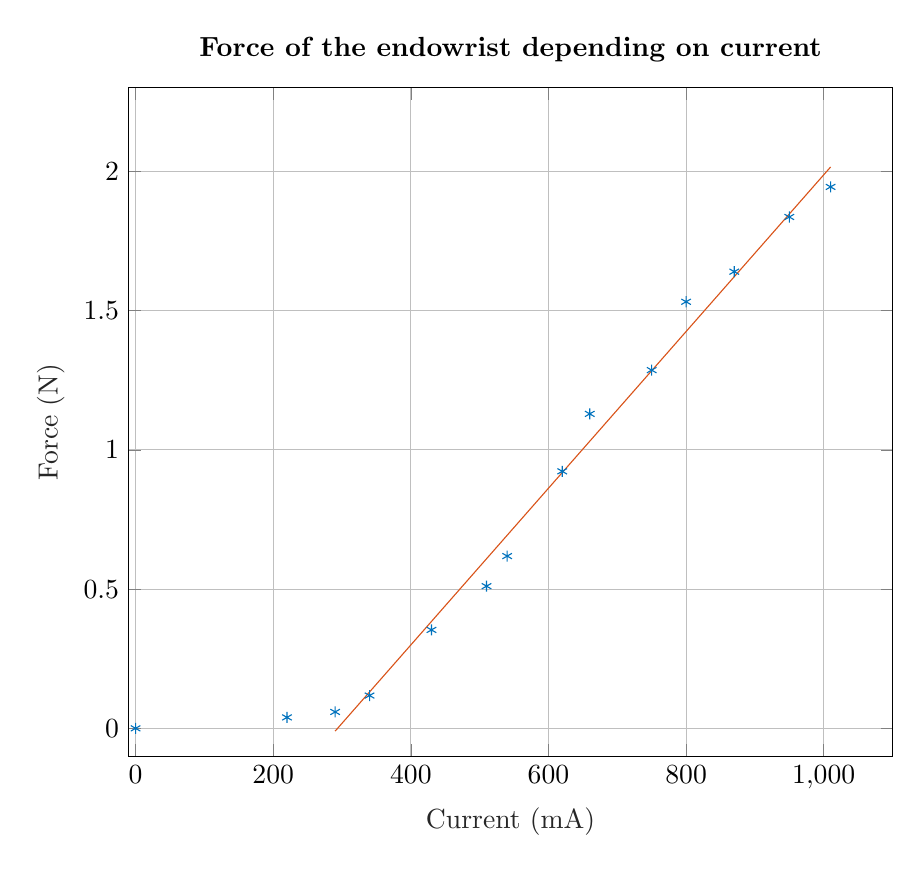
\begin{tikzpicture}

\begin{axis}[%
width=0.8\columnwidth,%7.484in,
height=0.7\columnwidth,%8.26in,
at={(0.758in,0.481in)},
scale only axis,
xmin=-10,
xmax=1100,
xlabel style={font=\color{white!15!black}},
xlabel={Current (mA)},
ymin=-0.1,
ymax=2.3,
ylabel style={font=\color{white!15!black}},
ylabel={Force (N)},
axis background/.style={fill=white},
title style={font=\bfseries},
title={Force of the endowrist depending on current},
xmajorgrids,
ymajorgrids
]
\addplot [color=mycolor1, draw=none, mark=asterisk, mark options={solid, mycolor1}, forget plot]
  table[row sep=crcr]{%
0	0\\
220	0.03928\\
290	0.05892\\
340	0.11784\\
430	0.35352\\
510	0.51064\\
540	0.61866\\
620	0.92308\\
660	1.1293\\
750	1.28642\\
800	1.53192\\
870	1.63994\\
950	1.83634\\
1010	1.94436\\
};
\addplot [color=mycolor2, forget plot]
  table[row sep=crcr]{%
290	-0.00996204344902341\\
340	0.130719594329395\\
430	0.383946542330548\\
510	0.609037162776017\\
540	0.693446145443068\\
620	0.918536765888537\\
660	1.03108207611127\\
750	1.28430902411242\\
800	1.42499066189084\\
870	1.62194495478063\\
950	1.8470355752261\\
1010	2.0158535405602\\
};
\end{axis}
\end{tikzpicture}%
\caption{The force measurements from the end-effector}
\label{endo_force_mes}
\end{figure}

\subsection*{Uncertainties of measurement:}
\begin{itemize}
\item Not 100 \% orthogonal force to the load cell.
\item Input/Output impedance of sensors have a $\pm 10 \%$ tolerance.
\item Movement of test setup when force is generated.
\end{itemize}

\subsection*{Conclusion:}
\todo{conclusion}